\documentclass[9pt,twoside,lineno]{pnas-new}
% Use the lineno option to display guide line numbers if required.

%% Packages 
\usepackage{longtable}
\usepackage{csvsimple}

%% shortcuts
\newcommand{\afb}{\mathsf{afb}}
\newcommand{\mic}{\mathsf{mic}}
\newcommand{\mol}{\mathsf{mol}}
\newcommand{\logplus}{\mathsf{log1}}


\templatetype{pnassupportinginfo}
% \readytosubmit %% Uncomment this line before submitting, so that the instruction page is removed.

\title{Association of Ebolavirus spillover events and annual birth pulses of African fruit bats}
\author{C. Reed Hranac, Jonathan C. Marshall, Ara Monadjem, David T. S. Hayman}
\correspondingauthor{David T. S. Hayman, E-mail: D.T.S.Hayman@massey.ac.nz}

\begin{document}

%% Comment/remove this line before generating final copy for submission
%\instructionspage  

\maketitle

%% Adds the main heading for the SI text. Comment out this line if you do not have any supporting information text.
\SItext


\section*{SI Methods}
\label{SI methods}

\subsection*{Chiropteran parturition data mining}
\label{dataMining}
Bat species that have been implicated in \textit{Filovirus} transmission either through RNA or antibody detection methods \cite{Han2016UndiscoveredFiloviruses,Walsh2005Wave-likeZaire} were systematically queried through Walker's Bats of the World \cite{Nowak1994WalkersWorld}, Scopus, Web of Science, and Google Scholar. Generalized search terms including: "Birth*"; "Breed*"; "Reproduc*"; "Partur*" along with the Latin binomial and common species names were used (bat species that had undergone taxonomic reassignment were queried under all names). Species that had been implicated, but did not reside in Africa, were queried at the genus level to identify representative sister species. Preliminary results suggested insufficient sample sizes to model parturition on a per-species basis and subsequently, the database was expanded to all mainland African bats. Species were then aggregated into three taxonomic clusters: African fruit bats (family: \textit{Pteropodidae}), molossid bats (family: \textit{Molossidae}, and non-molossid microbats, according to \cite{Cumming1997RainfallBats}, to account for shared life history traits including those associated with reproductive strategies and dietary preferences. Publications were accessed by hand and the location and month of parturition events were extracted. Additional points for non-implicated species were added opportunistically as discovered and an African bat specialist (AM) was consulted to help fill holes in the dataset. All gathered data was then compiled into a single, recirculating year for further analysis.\par
\subsection*{Co-variate data}
\label{CoV}
Co-variate data was assembled to for both the bat birthing models and EVD spillover models and is summarized in Table~\ref{table:ENM_CoV}. Co-variate layers were blocked into static variables and temporally dynamic variables depending on the data availability and hypotheses being tested. The static co-variate layers used included those describing mammalian species biodiversity \cite{IUCN2016TerrestrialData}, land cover \cite{Olivier2012Global2009}, and four of the 19 Bioclimatic variables representing 30 year average for precipitation seasonality, mean diurnal range, temperature seasonality, and temperature annual range \cite{Frick2017WorldclimArease}. Temporally dynamic co-variate layers were used to describe mean monthly temperature, average monthly precipitation, potential evapo-transpiration \cite{Trabucco2009GlobalDatabase} and an enhanced vegetative index \cite{Huete2002OverviewIndices}.\par
Considering the vast size of Africa the study extent was restricted to locations in Africa receiving more than 500mL of precipitation annually as suggested by Schmidt \textit{et al.} 2017\cite{Schmidt2017SpatiotemporalSpillover}. All co-variate layers were cropped and  masked to the precipitation layer, resolution was aggregated to ~25km raster blocks and temporally dynamic co-variates were normalized (mean zero and standard deviation of 1). All spatial handling was preformed within R \cite{Team2017R:Computing}, using tools within the \texttt{sp}\cite{Pebesma2005ClassesR}, \texttt{raster}\cite{Hijmans2016Raster:Modeling}, and \texttt{rgdal}\cite{Bivand2017Rgdal:Library} packages.\par
\subsubsection*{Mammalian diversity layers}
Co-variate layers describing non-volant mammalian, African fruit bat, molossid, and non-Molossid microbats diversity were created using the IUCN red list terrestrial mammals distribution database \cite{IUCN2016TerrestrialData}. Classification by taxonomic rank was performed by \texttt{taxize} package \cite{Chamberlain2013Taxize:R} and manually checked by hand (see \texttt{DiversityRasters.R}) and the number of overlapping distributions for each cell within the study area were counted.\par
\subsubsection*{Land cover}
The global land cover database \cite{Olivier2012Global2009} was obtained for the year 2009 and custom aggregation was used to reduce the number of classes from 23 to five as described by Table~\ref{table:globReclass}.\par
\subsubsection*{Fragmentation index}
A binary mask of the aggregated `forest' class (as described above) from the Globcover 2009 dataset \cite{Olivier2012Global2009} was used to define forest patches using 4-connectivity. A fragmentation index was then calculated for each pixel by counting the number of unique patches within a 20x20 sliding window using tools in the \texttt{EBImage} package. \par
\subsection*{African bat birth pulse modeling}
\label{biomod}
The birth pulses of Chiropteran taxonomic clusters were modeled though a modified ecological niche modeling (ENM) procedure devised for this analysis. Standard ENMs use occurrence (or occurrence/absence) and co-variate data to create regressive correlations between observed environmental phenomena and observations. In this instance, we re-purposed these models to correlate phenological environmental signals with bat birthing events within a temporally dynamic framework.\par
Birthing events identified through the data mining were split by taxonomic grouping as described above and observation/absence matrices were generated using a sliding two month window. Records of a birth within the window were recorded as an occurrence and all locations for which data was present, but no births were recorded for that taxonomic group were deemed "absence points". The two month sliding window was chosen to reflect the non-discrete nature of birthing within wild animals and to help account for deficiencies in the source data. An additional ten, randomly generated, down-weighted points (five occurrence and five absence points) were added to all models to insure the representation of all land cover categories in all models, and provide necessary pseudo-absence points in a small number of cases in which and insufficient number of absence points existed.\par
Temporal co-variate data was selected using a wider six month sliding window. Selections were centred on the same two month sliding window used for the occurrence/absences and included the two preceding, and two following months. Due to the inherent correlation of the co-variate layers (especially the temporally dynamic co-variate layers) and general non-independence of all selected environmental metrics, a raster based princal components analysis (PCA) method was used to reduce the dimensionality of all continuous predictors into six orthogonal principal components using the \texttt{rasterPCA} function of the package RSToobox. The categorical land cover variable was then added back to the other dimensionally reduced co-variates and occurrence/absence data were fed into the \texttt{biomod2}\cite{Thuiller2017Biomod2:Modeling} framework.\par
EMNS were then procedurally generated for all taxonomic clusters for all pairs of consecutive months where the number of combined observations was greater than 7. Ten iterations of the potential eight preliminary models (generalized linear model, generalized boosted model, classification tree analysis, artificial neural network, surface range envelope, flexible discriminate analysis, random forest and maximum entropy) were computed using a standard 70:30 training:test ratio. Ensemble models were then compiled based on the weighted mean of the receiver operating characteristic (ROC score) to create a single consensus layer with the probability of event occurrence between 0 and 1.\par
\subsubsection*{Force of birthing}
Ensemble model results were combined with taxonomic beta diversity (as described above) to create a "Force of Birthing" (FoB) metric $\lambda_{T,i,t}$ to represent the relative number of members of each taxon $T \in \{\afb, \mic, \mol\}$ giving birth at any location in time and space as described by:
\[
  	    \lambda_{T,i,t} = \log(P(\mathsf{Birth}_{T,i,t})*\beta_{T,i} +1)
\]
where probability of birth occurrence is $P(\mathsf{Birth}_{T,i,t})$ for each taxonomic group $T$, at location $i$ and time $t$. The number of taxonomic members is give by $\beta_{T,i}$. The abbreviations $\afb$, $\mic$ and $\mol$ were used to represent African fruit bats, Non-Molossid Microbats, and Molossidae respectively. \par 
\subsection*{Modeling of EVD outbreak events}
\label{spatGLM}

To test our hypothesis that the annual birthing cycles of African bats influences the spillover of EVD wewe collapsed the 42 year history of EVD outbreaks into a single recirculating year, treating outbreaks as a spatio-temporal poisson point process, with rate (herein, risk) estimated using a spatially weighted, over dispersed general linear model (spatGLM). Forest dwelling animals susceptible to EVD presumably have different habitat use and contact patterns with the potential reservoir host(s) than humans and therefore spillover into non-human mammals were modeled independently of humans. Forest dwelling animals susceptible to EVD presumably have different habitat use and contact patterns with the potential reservoir host(s) than humans and therefore spillover into non-human spillover hosts were modeled independently of humans. Current hypotheses of filovirus spillover risk posit that synchronous shifts in population demographic may be responsible for periods of increased viral shedding \cite{Hayman2015BiannualPopulations, Pourrut2009LargeAegyptiacus.}. To include these, temporal lag terms of the FoB were included to test the period at which this may occur relative to the birth pulses. Risk of EVD spillover into non-reservoir animals was defined as:
\[
\begin{split}
    \log(R& _{\mathsf{an}, i, t}) \sim \\
    & \beta_1 \lambda_{\afb, i, t} + \beta_2 \lambda_{\mic, i, t} + \beta_3 \lambda_{\mol, i, t} \\
 + &\beta_4 \lambda_{\afb, i, t-2} + \beta_5 \lambda_{\mic, i, t-2} + \beta_6 \lambda_{\mol, i, t-2} \\
 + &\beta_7 \lambda_{\afb, i, t-4} + \beta_8 \lambda_{\mic, i, t-4} + \beta_9 \lambda_{\mol, i, t-4} \\
 + &\beta_{10} \lambda_{\afb, i, t-6} + \beta_{11} \lambda_{\mic, i, t-6} + \beta_{12} \lambda_{\mol, i, t-6} \\
 +&\beta_{13} \mathsf{BVD}_{i,t} +  \beta_{14} \logplus(\mathsf{NBM div}_{i})\\
 + &\beta_{15} \logplus(\mathsf{fragIndex}_{i}) 
\end{split}
\]
where $RR_{\mathsf{an}, i, t}$ represents the risk of EVD spillover at spatial location $i$, and month $t$. The FoB for each taxonomic cluster were included as $\lambda_{T, i, t}$, with temporal lags specified. Detection of ebolavirus within wild bats on the landscape were included by the term $\mathsf{BVD}_{i,t}$. Non-volant mammalian diversity, and a forest fragmentation were also included as the terms $\mathsf{NBM div}_{i}*$ and $\mathsf{fragIndex}_{i}*$. The transformation $\logplus(x) = \log(x + 1)$ was used to treat these variables on the log scale while allowing that they might be zero.

Human outbreak events are not exclusively linked to proposed reservoir host exposure \cite{Pourrut2005TheAfrica} and outbreaks within non-humans spillover hosts were included within the human spillover model to include these epidemic chains. An additional non-reservoir host term was included describe the stuttering epidemic chain from these animals while still taking into account the rapid progression of EVD to mortality \cite{Swanepoel1996ExperimentalVirus}. The risk of EVD spillover into humans ($RR_{hum}$) was described by:
\[
    \begin{split}
\log(RR&_{\mathsf{hum}, i, t}) \sim \\
&\beta_1 \lambda_{\afb, i, t} + \beta_2 \lambda_{\mic, l, i, t} + \beta_3 \lambda_{\mol, i, t} \\
 + &\beta_4 \lambda_{\afb, i, t-2} + \beta_5 \lambda_{\mic, i, t-2} + \beta_6 \lambda_{\mol, i, t-2} \\
 + &\beta_7 \lambda_{\afb, i, t-4} + \beta_8 \lambda_{\mic, i, t-4} + \beta_9 \lambda_{\mol, i, t-4} \\
 + &\beta_{10} \lambda_{\afb, i, t-6} + \beta_{11} \lambda_{\mic, i, t-6} + \beta_{12} \lambda_{\mol, i, t-6} \\
 + &\beta_{13} OB_{\mathsf{an}, i, t} + \beta_{14} OB_{\mathsf{an},i, t-1}  \\
 +&\beta_{15} \mathsf{BVD}_{i,t} + \beta_{16} \logplus(\mathsf{PopDen}_{i})  \\
 + &\beta_{17} \logplus(\mathsf{NBM div}_{i}) + \beta_{18} \logplus(\mathsf{fragIndex}_{i})  
    \end{split}
\]
Human population density, $\mathsf{PopDen}_{i}$ was included to represent the human-wildlife interface \cite{Plowright2015EcologicalSpillover.}.  \par
Null models were computed to test the contribution of bat associated terms to over all model fit and were of the form:
\[
\begin{split}
   \log(RR&_{\mathsf{hum}, i, t}) \sim \\ 
   &\beta_{1} OB_{\mathsf{an}, i, t} + \beta_{24} OB_{\mathsf{an}, i, t-1}  \\
 +&\beta_{3} \logplus(\mathsf{NBM div}_{i}) + \beta_{4} \logplus(\mathsf{PopDen}_{i})  \\
 + &\beta_{5} \logplus(\mathsf{fragIndex}_{i})
\end{split}
\]
and 
\[
\begin{split}
   \log(RR& _{\mathsf{an}, i, t}) \sim \\
   & \beta_1 \mathsf{NBM div_i} + \beta_2 \logplus(\mathsf{fragIndex}_{i})
\end{split}
\]

\subsection*{qAIC}
\label{qAIC}
Models with and without bat associated terms were compared using a quasi-Akaike information criteria (qAIC) scheme of the form: 
\[
\mathsf{qAIC} = -2 \mathsf{logLik}/\hat{C} + 2k,
\]
where $\hat{C}$ is the overdispersion, and $k$ represents the number of terms in the model.\\


%%% Each figure should be on its own page

%% Long table start
\newpage\clearpage
\setlength\tabcolsep{3.3pt}
\begin{longtable}{cccp{5cm}}
\caption{African bat birth pulse data mining results}\label{table:DataMining}\\
\multicolumn{1}{c}{\textit{Species}} & \multicolumn{1}{c}{Annual Births} & \multicolumn{1}{c}{Locations} & \multicolumn{1}{c}{References}\\
\hline 
\endfirsthead

\multicolumn{3}{c}%
{{\bfseries \tablename\ \thetable{} -- continued from previous page}} \\
\hline \multicolumn{1}{c}{\textit{Species}} & \multicolumn{1}{c}{Number Annual Births} & \multicolumn{1}{c}{Number Locations} & \multicolumn{1}{c}{References}\\ \hline 
\endhead

\hline \multicolumn{3}{|r|}{{Continued on next page}} \\ \hline
\endfoot

\hline \hline
\endlastfoot
\multicolumn{4}{l}{\textit{Pteropodidae}} \\
\hline \hline
\textit{Casinycteris ophiodon} & 1 & 1 & \cite{Wolton1982EcologicalMicrochiroptera} \\
\textit{Eidolon helvum} & 1-2 & 3 & \cite{Mutere1967The020N,Thomas1983ThePteropodidae,Funmilayo1979ECOLOGYNIGERIA,Fayenuwo1974BreedingNigeria}\\
\textit{Epomophorus gambianus} & 1-2 & 3 & \cite{COE1975MAMMALIANLIBERIA,Marshall1982EcologicalWoodland,Thomas1984ReproductionBats}\\
\textit{Epomophorus labiatus} & 2 & 1 & \cite{Okia1974TheUganda.}\\
\textit{Epomophorus wahlbergi} & 1-2 & 2 & \cite{Monadjem2012BreedingSwaziland,Wickler1976FieldCalling.}\\
\textit{Epomopos buettikoferi} & 2 & 2 & \cite{Thomas1984ReproductionBats,Kofron1994ReproductionLiberia}\\
\textit{Epomopos franqueti} & 2 & 3 & \cite{Bergmans1979TaxonomyMegachiroptera,King2010TheCongo,Okia1974TheUganda.}\\
\textit{Hypsignathus monstrosus} & 2 & 3 & \cite{Bradbury2010LekBat,Kingdon1974EastBats,Wolton1982EcologicalMicrochiroptera}\\
\textit{Micropteropus pusillus} & 1-2 & 6 & \cite{Bergmans1976AMegachiroptera,Okia1987ReproductiveBats,Verschuren1957EcologieChiropteres,Marshall1982EcologicalWoodland,Hill1971BatsExpedition,Thomas1984ReproductionBats}\\
\textit{Myonycteris angolensis} & 1 & 2 & \cite{COE1975MAMMALIANLIBERIA,Wolton1982EcologicalMicrochiroptera}\\
\textit{Myonycteris leptodon} & 1-2 & 3 & \cite{Thomas1983ThePteropodidae,Wolton1982EcologicalMicrochiroptera}\\
\textit{Myonycteris torquata} & 2 & 1 & \cite{Bergmans1976AMegachiroptera}\\
\textit{Nanonycteris veldkampi} & 1	& 2	& \cite{Wolton1982EcologicalMicrochiroptera,Marshall1982EcologicalWoodland}\\
\textit{Rousettus aegyptiacus} & 1-2 & 12 & \cite{Wolton1982EcologicalMicrochiroptera,Marshall1982EcologicalWoodland,Herzig-Straschil1978OnPark,Jacobsen1976ObservationsTransvaal,Adam1974LesParasitologiques,Kingdon1974EastBats,Okia1987ReproductiveBats,COE1975MAMMALIANLIBERIA,Anderson1902ZoologyMammalia,Mutere1968TheSouth}\\
\hline 
\multicolumn{4}{l}{\textit{Molossidae}} \\
\hline \hline
\textit{Chaerephon pumilas} & 2-3 & 4 & \cite{vanderMerwe1987AdaptiveS,Happold1989ReproductionAfrica.,MUTERE1973ReproductionMolossidae,Mcwilliam1987TheEnvironment}\\
\textit{Chaerephon pumilus} & 1 & 1 & \cite{Monadjem1998NotesRecords}\\
\textit{Mops condylurus} & 2 & 5 & \cite{Vivier2001AspectsAfrica,Happold1989ReproductionAfrica.,OShea1980EcologicalCommunity,MUTERE1973ReproductionMolossidae}\\
\textit{Mops midas} & 1 & 1 & \cite{Smithers1971TheBotswana}\\
\textit{Otomops harrisoni} & 1 & 2 & \cite{MUTERE1973ReproductionMolossidae}\\
\textit{Tadarida aegyptiaca} & 1 & 1 & \cite{Bernard1995SeasonallyTemperate...}\\
\textit{Tadarida fulminans} & 2 & 1 & \cite{Cotterill1993SeasonallyZimbabwe}\\
\hline
\multicolumn{4}{l}{Non-\textit{Molossidae} Microbats} \\
\hline \hline
\textit{Cardioderma cor} & 2 & 1 & \cite{Vaughan1976NocturnalCor}\\
\textit{Coleura afra} & 2 & 1 & \cite{Mcwilliam1987TheEnvironment}\\
\textit{Eptesicus hottentotus} & 1 & 1 & \cite{Happold2013MammalsBats}\\
\textit{Hipposideros abae} & 1 & 1 & \cite{Verschuren1957EcologieChiropteres}\\
\textit{Hipposideros beatus} & 1 & 1 & \cite{Brosset1966LaChiropteres}\\
\textit{Hipposideros caffer} & 1 & 3 & \cite{Bernard1982FemaleAfrica,Ansell1986SomeAfrica,Menzies1973ANigeria}\\
\textit{Hipposideros caffer rubber} & 1 & 2 & \cite{Verschuren1957EcologieChiropteres,Wolton1982EcologicalMicrochiroptera}\\
\textit{Hipposideros cyclops
} & 1 & 1 & \cite{Verschuren1957EcologieChiropteres}\\
\textit{Hipposideros gigas} & 1 & 2 & \cite{Mcwilliam1982AdaptiveKenya,Brosset1969LaGabon}\\
\textit{Hipposideros rubber} & 1 & 1 & \cite{Howell1976AnTanzania}\\
\textit{Hipposideros vittatus} & 1 & 1 & \cite{Cotterill1999ReproductiveConservation}\\
\textit{Lavia frons} & 1 & 2 & \cite{Verschuren1957EcologieChiropteres,Vaughan1986SeasonalityYellow-Winged}\\
\textit{Miniopterus fraterculus} & 1 & 1 & \cite{Bernard1980Reproductive1906}\\
\textit{Miniopterus inflatus} & 1 & 1 & \cite{Brosset1969LaGabon}\\
\textit{Miniopterus minor} & 1 & 1 & \cite{McWilliam1988TheTropics}\\
\textit{Miniopterus natalensis} & 1 & 4 & \cite{Bernard1996OnZimbabwe,Bernard1980Reproductive1906,Bernard1994EffectsSchreibersii.,vanderMerwe1979FoetalNatalensis}\\
\textit{Myotis bocageii} & 2 & 1 & \cite{Brosset1966LaChiropteres}\\
\textit{Myotis tricolor} & 1 & 1 & \cite{Bernard1981MonthlyChiroptera}\\
\textit{Neoromicia capensis} & 1 & 1 & \cite{vanderMerwe1994ReproductiveAfrica}\\
\textit{Neoromicia nanus} & 1 & 4 & \cite{vanderMerwe2006Aspects1833,LaVal1977ReproductionNanus,Bernard1997SpermMalawi,OShea1980EcologicalCommunity}\\
\textit{Neoromicia somalicus} & 1 & 1 & \cite{OShea1980EcologicalCommunity}\\
\textit{Neoromicia zuluensis} & 1 & 1 & \cite{Happold1990ReproductiveAfrica}\\
\textit{Nycteris grandis} & 1 & 1 & \cite{FENTON1987ForagingZimbabwe}\\
\textit{Nycteris hispidar} & 2 & 1 & \cite{Verschuren1957EcologieChiropteres}\\
\textit{Nycteris nana} & 1 & 1 & \cite{Verschuren1957EcologieChiropteres}\\
\textit{Nycteris thebaica} & 1 & 1 & \cite{Bernard1982FemaleAfrica}\\
\textit{Nycticeinops schlieffeni} & 1 & 3 & \cite{VanderMerweN.J.Rautenbach1988AVespertilionidae,OShea1980EcologicalCommunity,Happold1990ReproductiveAfrica}\\
\textit{Pipistellus rusticus} & 1 & 1 & \cite{vanderMerwe1990ReproductionAfrica.}\\
\textit{Rhinolophus basii} & 1 & 1 & \cite{Happold1990ReproductiveAfrica}\\
\textit{Rhinolophus capensis} & 1 & 1 & \cite{Bernard1983ReproductionAfrica}\\
\textit{Rhinolophus clivossis} & 1 & 1 & \cite{Bernard1983ReproductionAfrica}\\
\textit{Rhinolophus darlingi} & 1 & 1 & \cite{Smithers1979CheckRhodesia}\\
\textit{Rhinolophus fumigatus} & 1 & 1 & \cite{Happold1990ReproductiveAfrica}\\
\textit{Rhinolophus landeri} & 1 & 1 & \cite{Menzies1973ANigeria}\\
\textit{Rhinolophus mossambicus} & 1 & 1 & \cite{Cotterill1998FemaleZimbabwe}\\
\textit{Rhinolophus simulator} & 1 & 2 & \cite{Cotterill1998FemaleZimbabwe,OShea1980EcologicalCommunity}\\
\textit{Scotoecus hirundo} & 1 & 1 & \cite{OShea1980EcologicalCommunity}\\
\textit{Scroptophilus borbonicus} & 1 & 1 & \cite{VanderMerweN.J.Rautenbach1988AVespertilionidae}\\
\textit{Scroptophilus dinganii} & 1-2 & 3 & \cite{OShea1980EcologicalCommunity,vanderMerwe2006Aspects1833,Okia1987ReproductiveBats}\\
\textit{Scroptophilus leucigaster} & 1 & 1 & \cite{Barclay1985NoLeucogastere}\\
\textit{Scroptophilus vividis} & 1 & 1 & \cite{VanderMerweN.J.Rautenbach1988AVespertilionidae}\\
\textit{Taphozous hildegardeae} & 2 & 1 & \cite{McWilliam1988TheTropics}\\
\textit{Taphozous mauritianus} & 2 & 2 & \cite{Happold1990ReproductiveAfrica,OShea1980EcologicalCommunity}\\
\end{longtable}
\FloatBarrier

%%%
\begin{table}
\centering
\caption{Co-variate layers for modelling}
\label{table:ENM_CoV}
\begin{tabular}{l c c r}
\multicolumn{1}{c}{Description} & \multicolumn{1}{c}{Analysis} & \multicolumn{1}{c}{Variable Type} & \multicolumn{1}{c}{References}\\
\hline\hline
Non-volant mammalian biodiversity & Both & Static & \cite{IUCN2016TerrestrialData}\\
Land cover (modified) & Both & Static & \cite{Olivier2012Global2009}\\
Precipitation seasonality & ENM & Static & \cite{Frick2017WorldclimArease}\\
Mean diurnal range & ENM & Static & \cite{Frick2017WorldclimArease}\\
Temperature seasonality & ENM & Static & \cite{Frick2017WorldclimArease}\\
Temperature annual range & ENM & Static& \cite{Frick2017WorldclimArease}\\
Mean monthly temperature & ENM & Temporal & \cite{Frick2017WorldclimArease}\\
Mean monthly precipitation & ENM & Temporal & \cite{Frick2017WorldclimArease}\\
Potential evapo-transpiration & ENM & Temporal & \cite{Trabucco2009GlobalDatabase}\\
Enhanced vegetative index & ENM & Temporal & \cite{Huete2002OverviewIndices}\\
Vegetation fragmentation index & spatGLM & Static & This study \\
Human population density & spatGLM & Static & \cite{CIESIN2005GriddedGrid}\\
\end{tabular}
\end{table}
\FloatBarrier

%%%
\begin{table}[!h]
\centering
\caption{Reclassification of land cover variables}
\label{table:globReclass}

\csvreader[tabular = l l l,
	table head = Value & Label & Class \\\hline\hline,
    late after line = \\,
    late after last line = \\\hline]%
    {globReclassSimple.csv}{Value =\Value,Label =\Label,Class =\Class}%
    	{\Value & \Label & \Class}%
\end{table}

%%%
\newpage\clearpage
\begin{table}[!h]
\centering
\caption{Ecological niche model ensemble scores.\\
The abbreviations ptr, mic, and mol, represent African fruit bats, non-molossid microbats and molissid bats respectively. The numbers included within the model names are the calender months over which the model was produced. No models were created for January-February, and July-August for the non-molossid microbats.}
\label{table:ENM_Scores}
\csvreader[tabular = l c c c,
	table head = Model & ROC & Sensitivity & Specificity \\\hline\hline,
    late after line = \\,
    late after last line = \\\hline]%
    {EMN_ModelResults.csv}{Model=\Model,ROC =\ROC,Sensitivity=\Sensitivity,Specificity=\Specificity}%
    {\Model & \ROC & \Sensitivity & \Specificity}%
    
\end{table}
\FloatBarrier

%%%
\newpage\clearpage
\begin{table}[!h]
    \centering
    \caption{Model comparison by qAIC\\
    Null models included no information of bat births or viral detection made within bats. $RRhum$ and $RRan$ are the risk of EVD spillover into humans and non-humans spillover hosts respectively}
    \label{tab:qAIC}
    \begin{tabular}{l r r r r}
    \multicolumn{1}{c}{Model} & \multicolumn{1}{c}{$k$} & \multicolumn{1}{c}{$\hat{C}$} & \multicolumn{1}{c}{$\mathsf{qAIC}$} & \multicolumn{1}{c}{$\Delta \mathsf{qAIC}$}\\
     \hline\hline
$RR_\mathsf{hum} Null$ & 6 & 1.88 & 1072.44 & - \\
$RR_\mathsf{hum} Full$ & 18 & 1.35 & 759.05 & -313.39 \\
$RR_\mathsf{an} Null$ & 3 & 1.04 & 423.91 & - \\
$RR_\mathsf{an} Full$ & 16 & 0.81 & 423.91 &  -93.54 \\    
    \end{tabular}
\end{table}

\newpage\clearpage
\begin{figure}
    \centering
    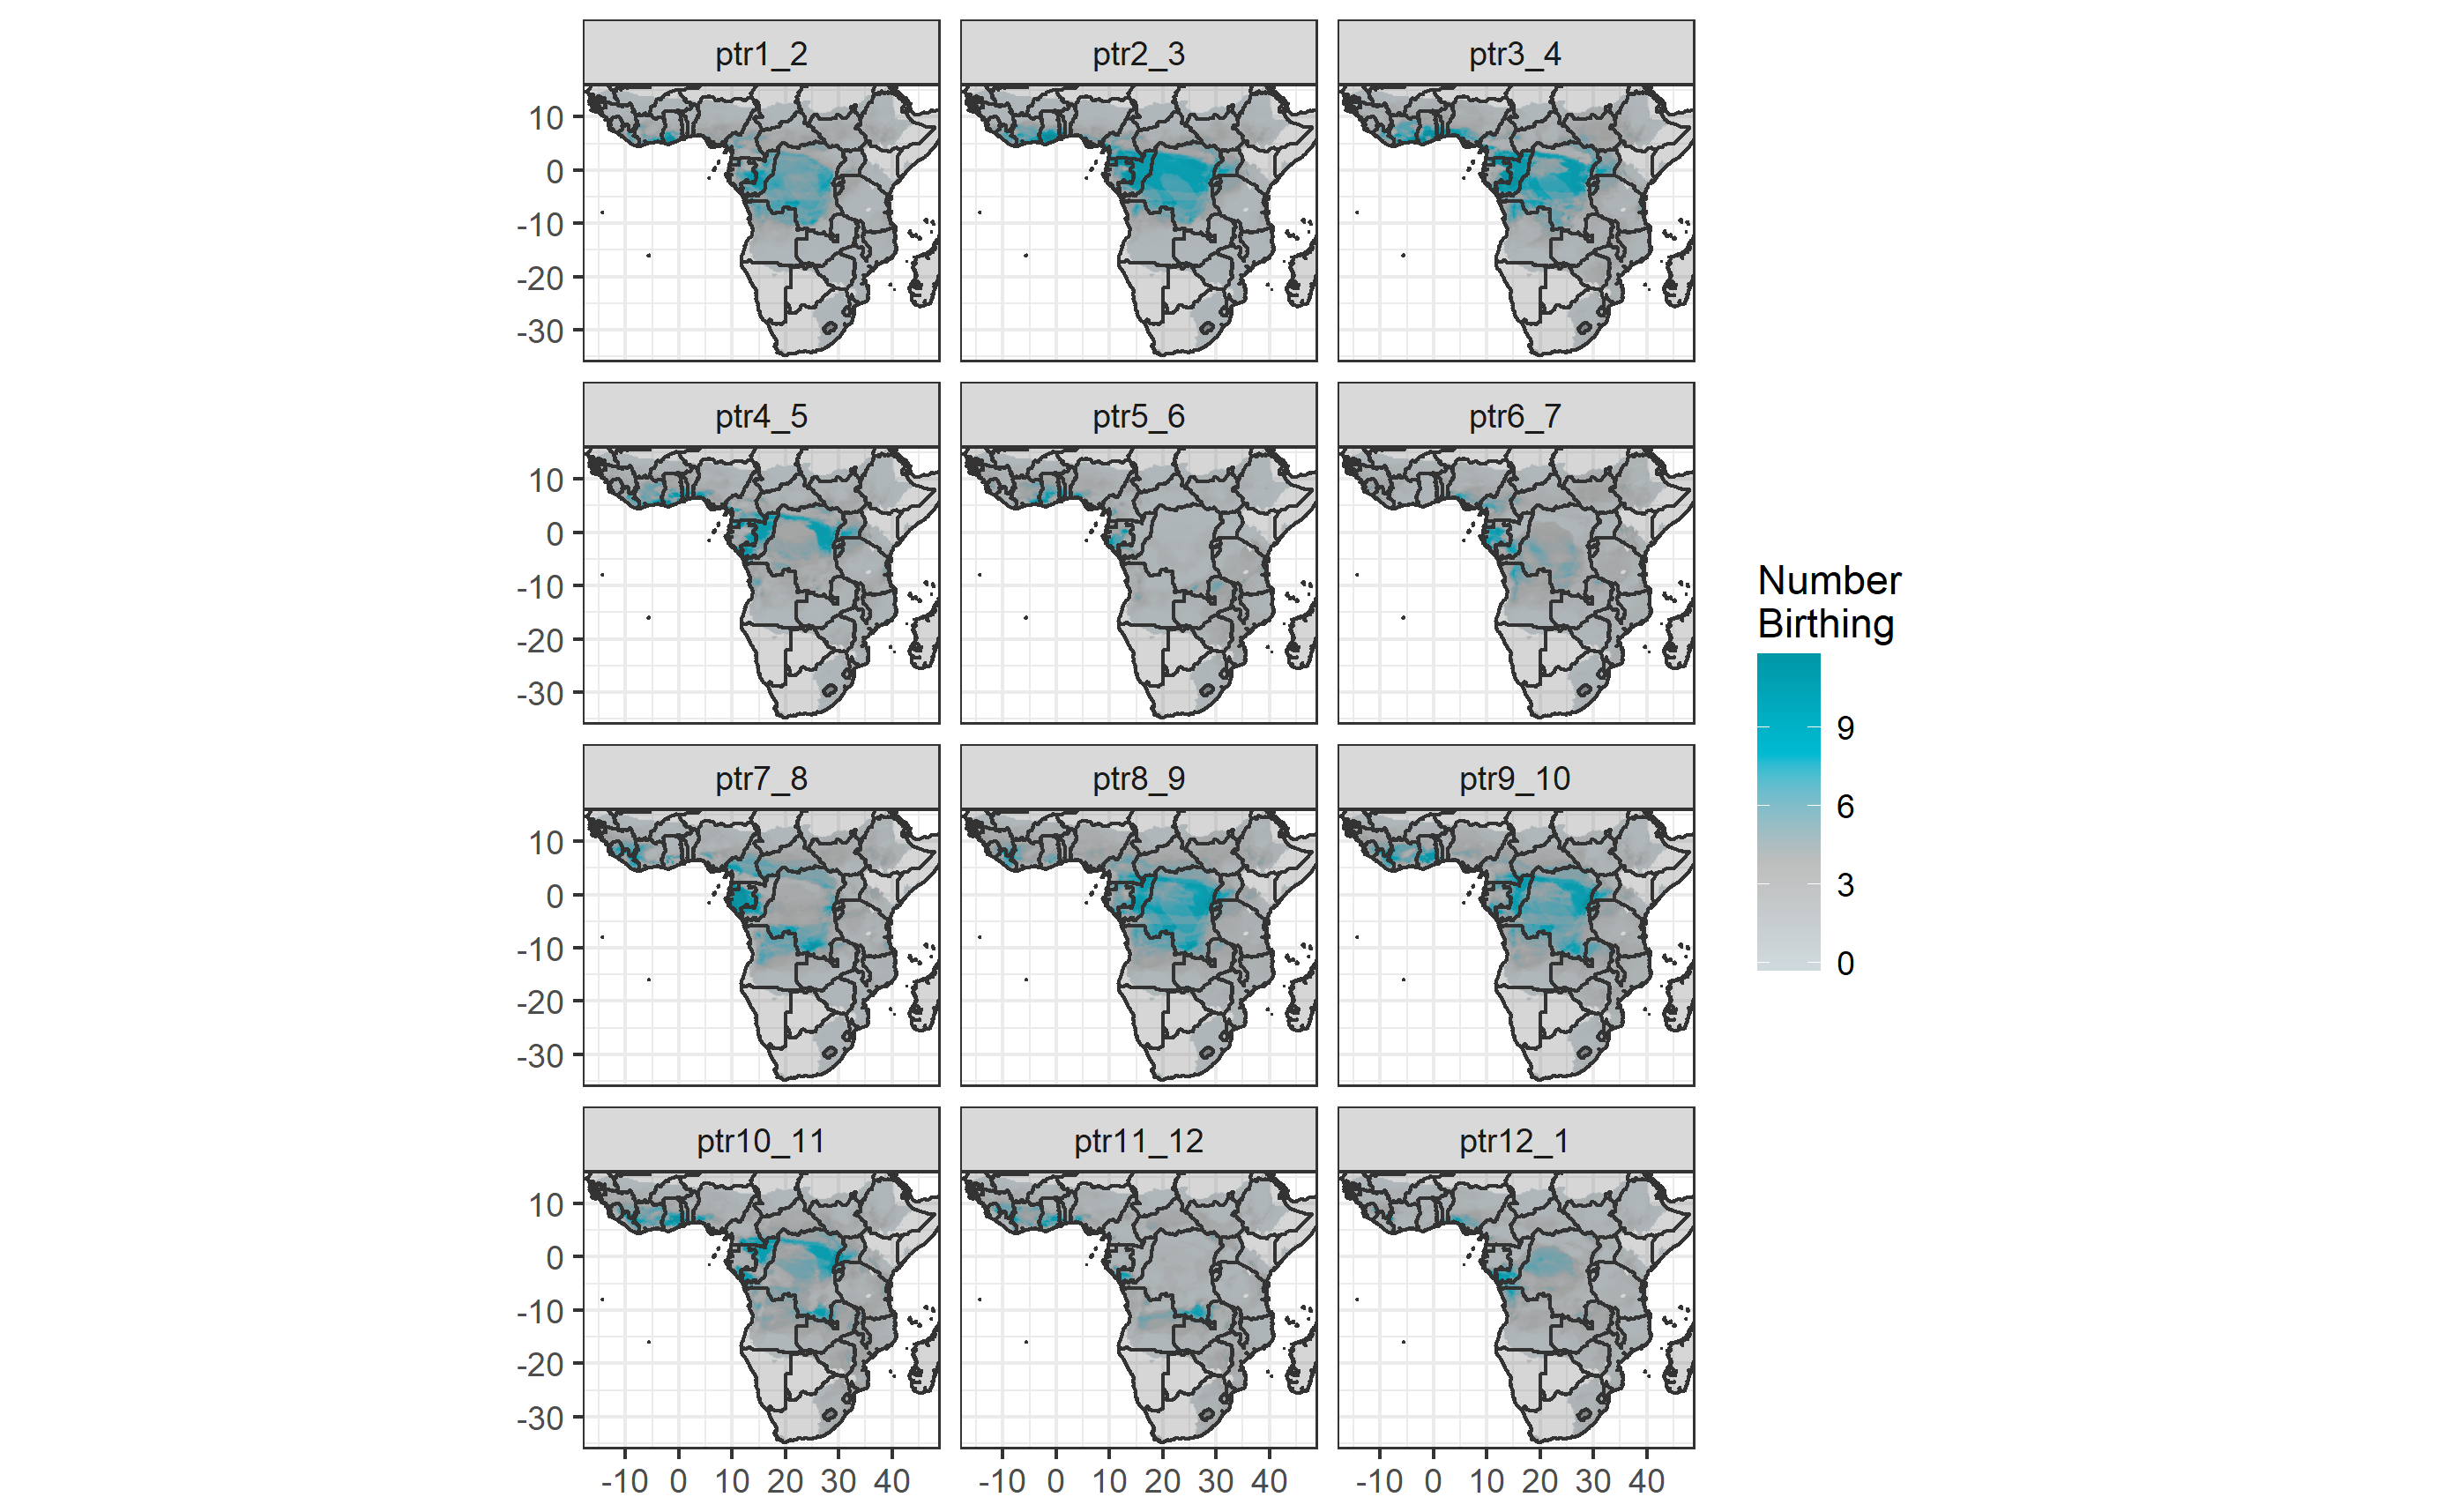
\includegraphics[width=.95\linewidth]{ptrBF_SI.pdf}
    \caption{Monthly force of birthing of African fruit bats}
    \label{fig:ptrBF}
\end{figure}
\FloatBarrier

\newpage\clearpage
\begin{figure}
    \centering
    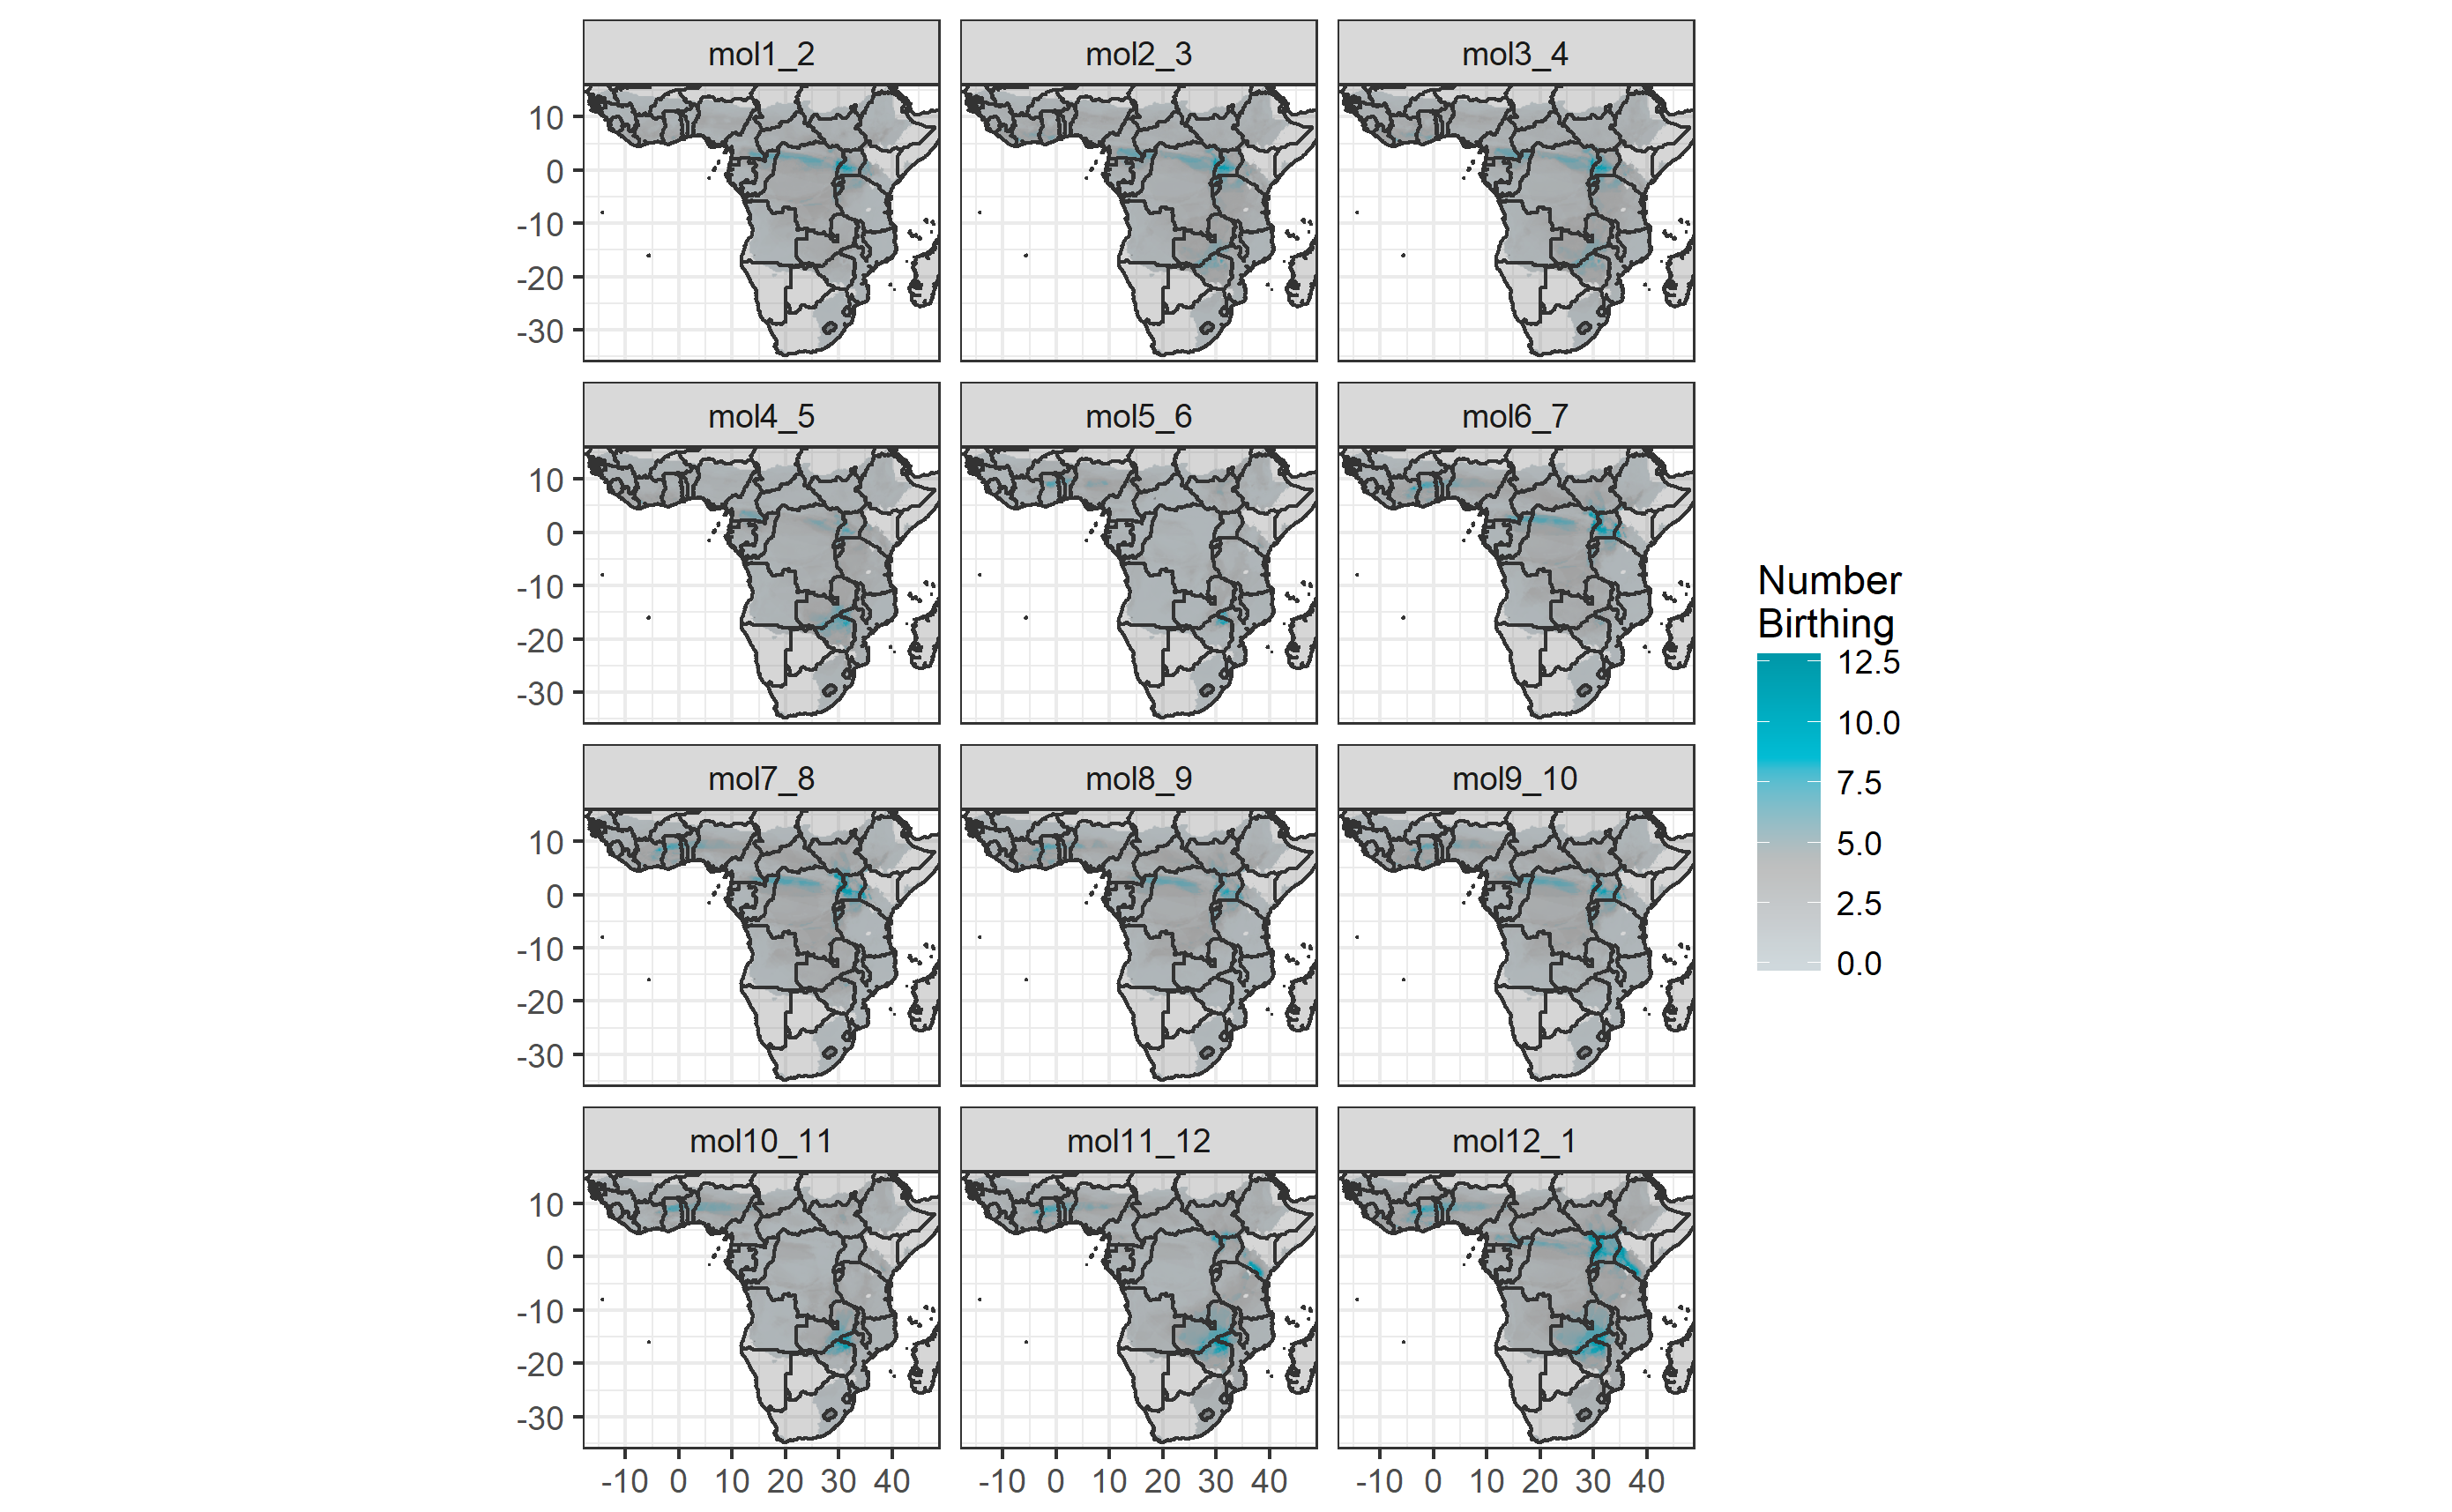
\includegraphics[width=.95\linewidth]{molBF_SI.pdf}
    \caption{Monthly force of birthing of molossid bats}
    \label{fig:molBF}
\end{figure}
\FloatBarrier

\newpage\clearpage
\begin{figure}
    \centering
    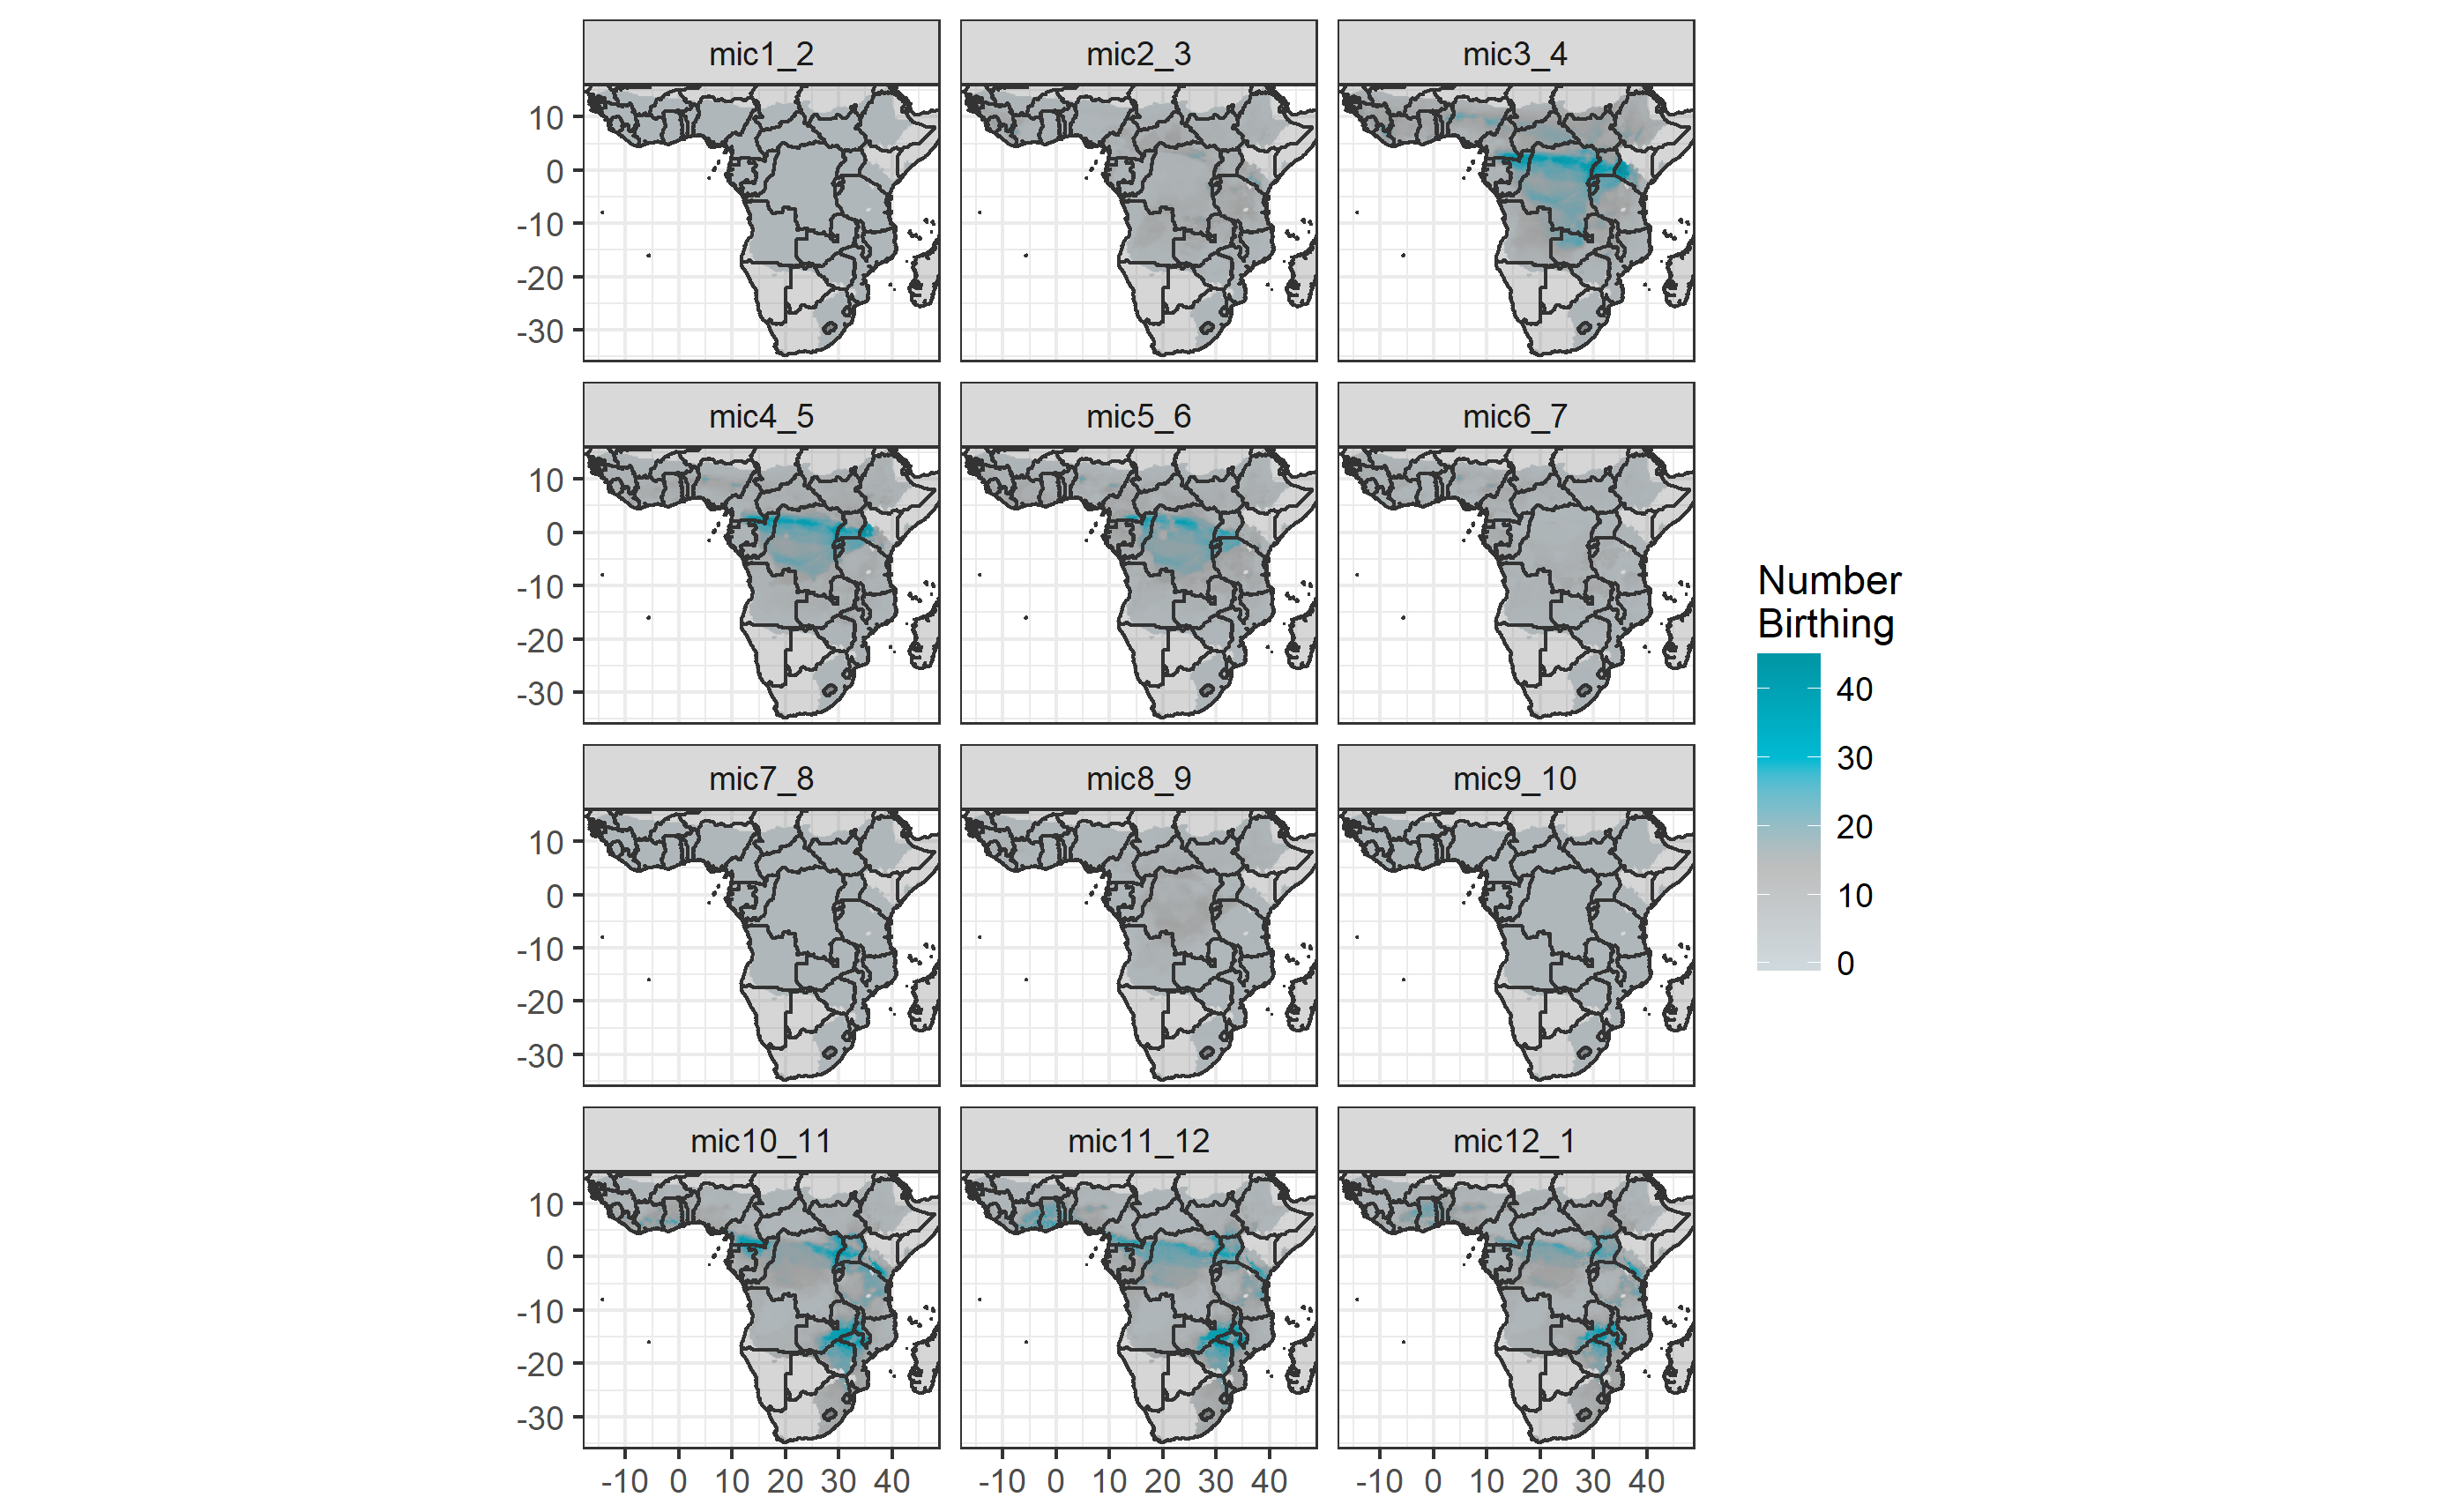
\includegraphics[width=.95\linewidth]{micBF_SI.pdf}
    \caption{Monthly force of birthing of non-molossid microbats. No models were generated for January-February or July-August.}
    \label{fig:micBF}
\end{figure}
\FloatBarrier

\newpage\clearpage
\begin{figure}
    \centering
    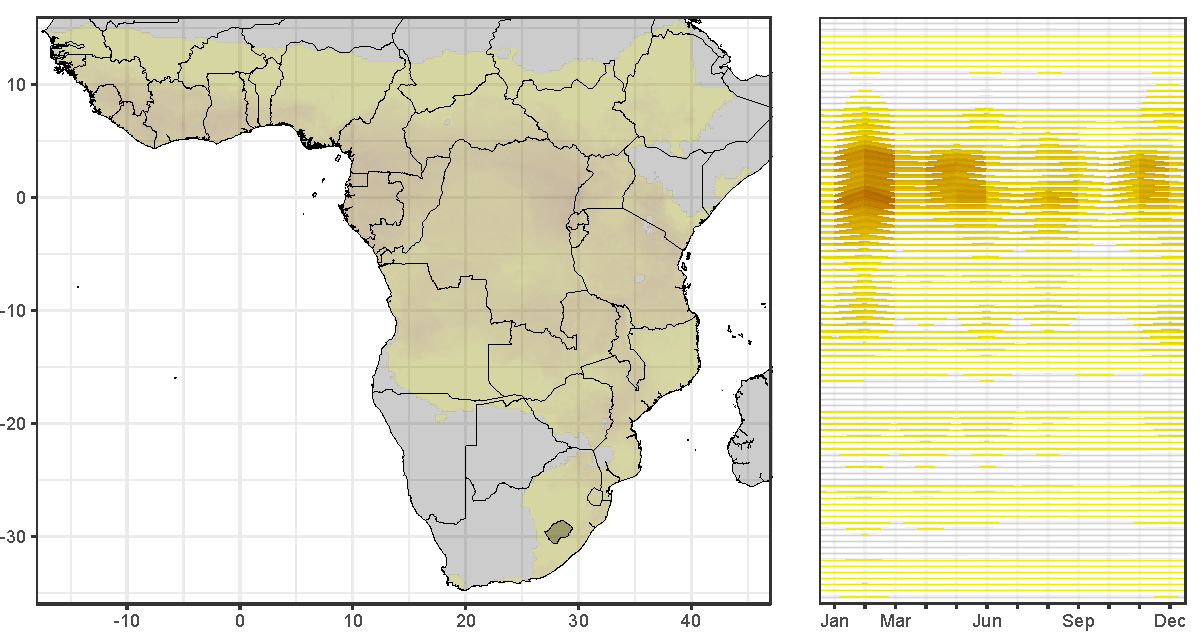
\includegraphics[width=.95\linewidth]{AnnRisk.pdf}
    \caption{\textit{Left:} Mean risk of EVD spillover to non-human reservoir hosts. \textit{Right:} Risk of EVD spillover aggregated by latitude and month.}
    \label{fig:AnRisk}
\end{figure}
\FloatBarrier

\newpage\clearpage
\begin{figure}
    \centering
    \includegraphics[width=.95\linewidth]{annRisk_SI.pdf}
    \caption{Monthly risk of EVD spillover to non-human reservoir hosts}
    \label{fig:AnRiskMonthly}
\end{figure}
\FloatBarrier

\newpage\clearpage
\begin{figure}
    \centering
    \includegraphics[width=.95\linewidth]{humRisk_SI.pdf}
    \caption{Monthly risk of EVD spillover into humans}
    \label{fig:HumRiskMonthly}
\end{figure}
%%%

\begin{table}
\centering
\caption{Non-human spillover host full spatGLM model results}
\label{table:spatGLM_AN}
\csvreader[tabular = l r r r  c,
	table head = Coefficients & Estimate & Std. Error & t Value &  P Value \\\hline\hline,
    late after line = \\,
    late after last line = \\\hline]%
    {AnFullResults.csv}{}%
    {\csvcoli &  \csvcolii &  \csvcoliii &  \csvcoliv &  \csvcolv}
\end{table}
\FloatBarrier

\begin{table}
\centering
\caption{Human spillover null spatGLM model results}
\label{table:spatGLM_Hum_Null}
\csvreader[tabular = l r r r  c,
	table head = Coefficients & Estimate & Std. Error & t Value &  P Value \\\hline\hline,
    late after line = \\,
    late after last line = \\\hline]%
    {HumNull.csv}{}%
    {\csvcoli &  \csvcolii &  \csvcoliii &  \csvcoliv &  \csvcolv}
\end{table}
\FloatBarrier

\begin{table}
\centering
\caption{Non-human spillover host null spatGLM model results}
\label{table:spatGLM_AN_Null}
\csvreader[tabular = l r r r  c,
	table head = Coefficients & Estimate & Std. Error & t Value &  P Value \\\hline\hline,
    late after line = \\,
    late after last line = \\\hline]%
    {AnNullResults.csv}{}%
    {\csvcoli &  \csvcolii &  \csvcoliii &  \csvcoliv &  \csvcolv}
\end{table}
\FloatBarrier
%%% Add this line AFTER all your figures and tables
\FloatBarrier


\dataset{afrBatBirthDB.csv}{African bat birth records database.}

\dataset{AnOutbreakDB.csv}{Ebola virus outbreaks and detection among non-humans. }

\dataset{HumOutbreakDB.csv}{Ebola virus index cases among humans.}
\bibliography{SI_FS_PNAS.bib}

\end{document}